\section{2022.4版修订说明}

\subsection{2022年4月1日更新内容}

\begin{enumerate}[1、]
    \item 将字体打包进来,避免在Mac OS上出现缺失字体的问题
    \item 移植到Overleaf平台上\footnote{\url{https://github.com/jtzhpf/NUIST-Bachelor-Thesis-LaTeX-Template-v2022.4.git}}
\end{enumerate}

\subsection{2022年4月21日更新内容}


\begin{enumerate}[1、]
    \item 封面logo修改为eps格式,原pdf格式会在封面中插入其他数据(正常情况下肉眼不可见,但在部分浏览器深色模式下可见)
    \item 在cls文件中新增附录格式。
\end{enumerate}


\begin{figure}[htbp]
    \center
    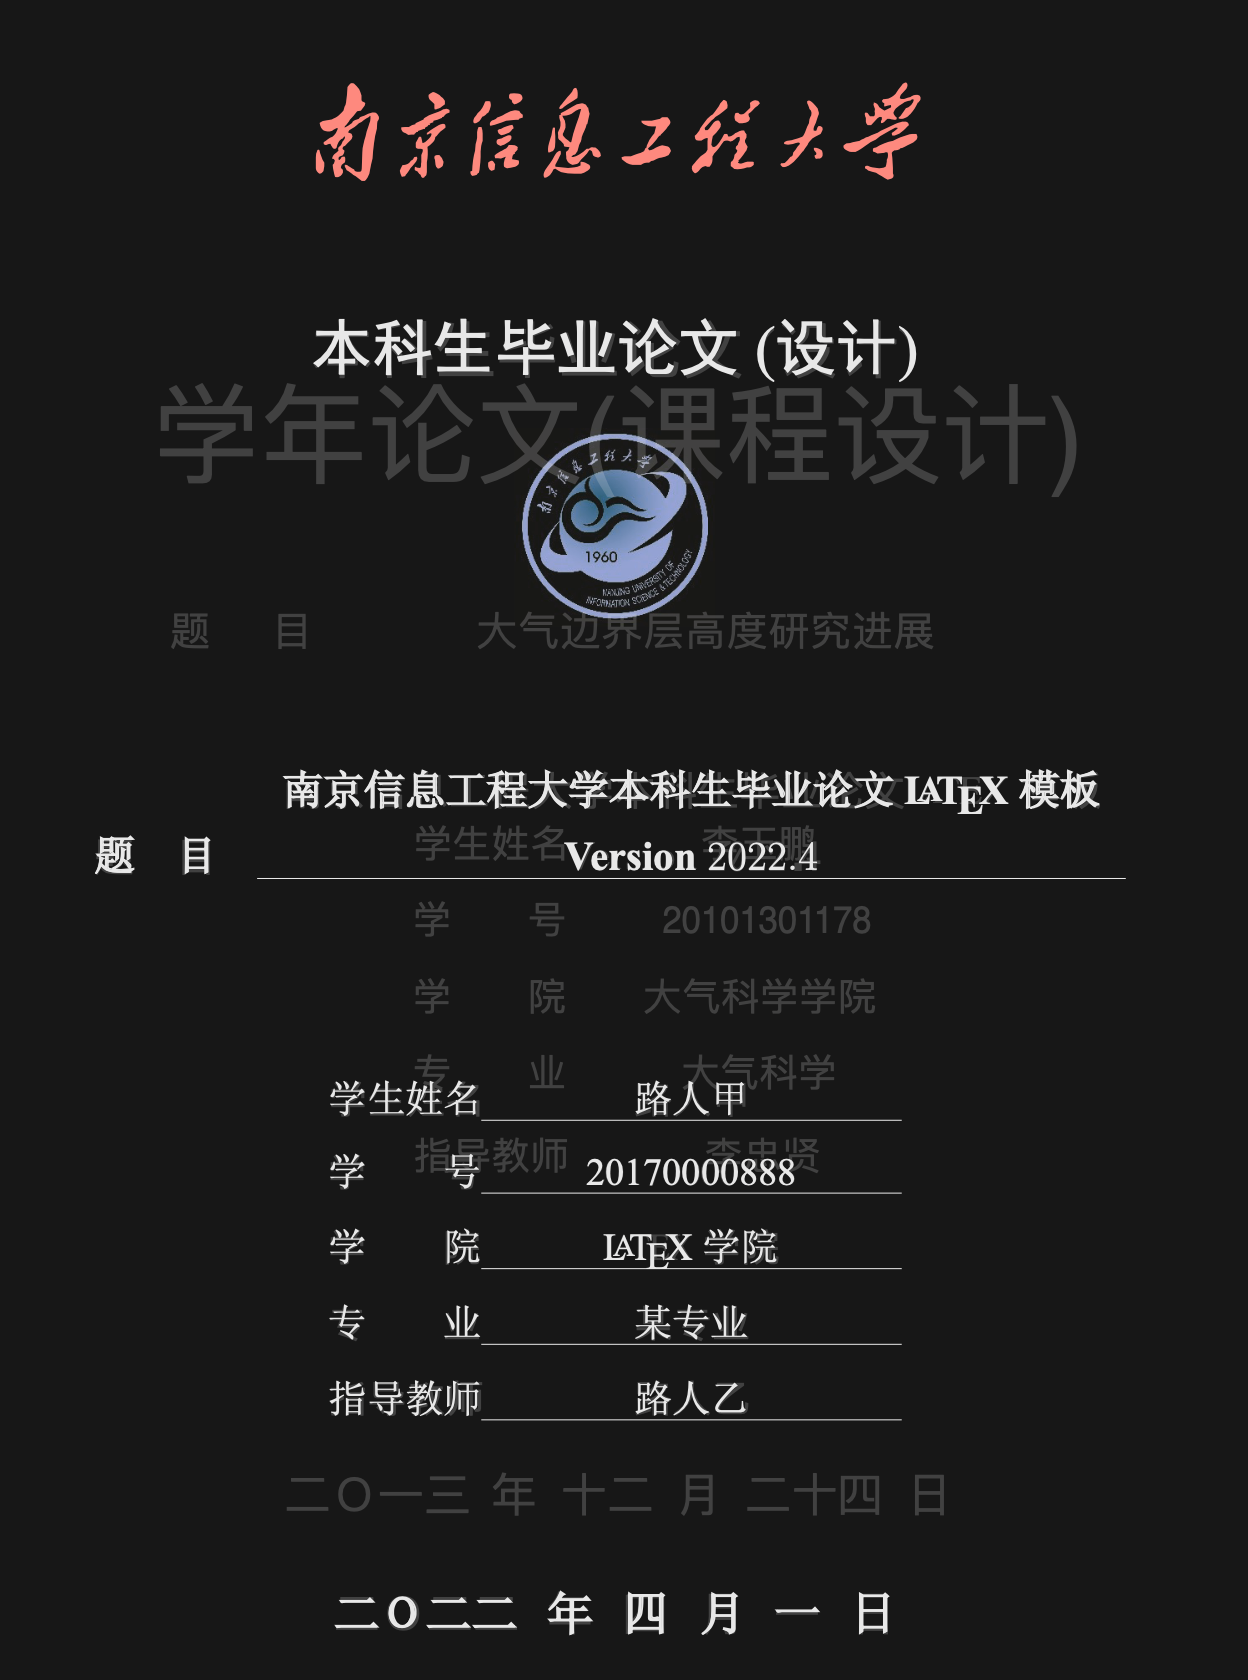
\includegraphics[width=0.5\textwidth]{figs/color/problem.png}
    \caption{pdf格式的logo带来的问题}
    \label{fig:problem}
\end{figure}


\subsection{致谢}
感谢本模版的制作者、2.0版修订者、3.1版制作者和2022版修订者,得益于你们的工作,才使得像我这样的小白也能轻松使用\LaTeX 编写毕业论文,本次修订的工作仅仅只是在前面各位工作的基础上做了一个跨平台(Mac OS和Overleaf)的适配。